% ConfPert: ICML 2026 Workshop on Hypothesis Testing submission (short paper, 4-page body).
% Per pre-registration outcome dispositions: K1 + K3 lead, K2 honest mixed
% result with one significant dataset (Replogle RPE1 H1 PASS).
% Workshop topical fit: (a) finite-sample distribution-free coverage = testing primitive,
% (b) pre-registered Spearman + permutation test with BH-FDR for K2,
% (c) BH-FDR multiple-testing correction over compound x pathway grid for K3,
% (d) cross-cell-line transfer = evaluation under distribution shift.

\documentclass{article}

% Recommended, but optional, packages for figures and better typesetting.
\usepackage{microtype}
\usepackage{graphicx}
\usepackage{subcaption}
\usepackage{booktabs}
\usepackage{hyperref}

% ICML 2026 style file (blind submission by default; the style auto-redacts
% author info on compile unless [accepted] is passed).
\usepackage{icml2026}

\usepackage{amsmath}
\usepackage{amssymb}
\usepackage{mathtools}
\usepackage{amsthm}
\usepackage{xcolor}

\newtheorem{proposition}{Proposition}

% Identity gate: blind by default. Set \camerareadytrue (and pass [accepted]
% to icml2026) for the non-blind camera-ready so the repository URL appears.
\newif\ifcameraready
\camerareadyfalse

% ICML running title (short form for header)
\icmltitlerunning{ConfPert: Conformal Coverage for Perturbation Predictors}

\begin{document}

\twocolumn[
\icmltitle{ConfPert: Distribution-Free Conformal Coverage \\ for Single-Cell Perturbation Predictors}

\icmlsetsymbol{equal}{*}

\begin{icmlauthorlist}
\icmlauthor{Aayan Alwani}{ind}
\end{icmlauthorlist}

\icmlaffiliation{ind}{Independent Researcher, USA}

\icmlcorrespondingauthor{Aayan Alwani}{alwaniaayan6@gmail.com}

\icmlkeywords{hypothesis testing, conformal prediction, distribution-free coverage, multiple testing, distribution shift, single-cell perturbation, calibration, Perturb-seq}

\vskip 0.3in
]

% This call ensures that the proper formatting commands are loaded for
% the submission and prints a footer indicating that the paper is
% under review unless [accepted] is passed.
\printAffiliationsAndNotice{}
% Fix: icml2026.sty's running-title auto-measurement (\ht\titrun>6.25pt) misfires
% for any normal-height title under this engine and substitutes the
% "Title Suppressed Due to Excessive Size" fallback. Re-assert the real running
% title after \icmltitle so the page header is correct. No style-file edit.
\makeatletter\gdef\@icmltitlerunning{ConfPert: Conformal Coverage for Perturbation Predictors}\makeatother

\begin{abstract}
Single-cell perturbation predictors are typically evaluated on mean-prediction metrics, but recent work shows that deep-learning foundation models systematically underperform a simple bilinear ridge baseline on these metrics \citep{ahlmann2025, csendes2025}, and no existing method provides coverage guarantees on the distributional fit between predicted and observed cell populations. We introduce \textbf{ConfPert}, a model-agnostic conformal prediction framework that gives finite-sample coverage guarantees on six per-population distributional discrepancies, exposed at four head levels: per-gene, per-perturbation, per-population, and subgroup-conditional. We use ConfPert to evaluate eight perturbation predictors spanning $0$ to $\sim 6 \times 10^8$ parameters across five single-cell datasets, including a cross-cell-line transfer split. The protocol is pre-registered: hypotheses, permutation-test thresholds, and multiple-comparisons corrections are committed to git before any first run. On Norman, the sparse-additive sVAE+ attains exact nominal coverage on the two variance-sensitive metrics (bimodality match and variance ratio), which mean-only predictors miss because a centroid prediction carries no within-population variance. The pre-registered capacity-hurts hypothesis fails its overall threshold: of the four pre-registered datasets only the non-cancer RPE1 line passes, and a post-registration fifth dataset (Tahoe-100M) passes only after the largest model is added. We report this as the honest null it is, alongside an exploratory association between the calibration--capacity trend and cell-line context. On real PRISM Repurposing drug-screen data, calibrated bimodal-subpopulation signatures show Benjamini-Hochberg-significant Hallmark enrichment well above a random-gene null, robustly across signature-size choices. We release a pip-installable \texttt{confpert} library and a Cell-Eval plug-in that adds the six discrepancies to Arc Institute's evaluation registry.
\end{abstract}

\section{Introduction}

\paragraph{The mean-only failure mode.}
Three independent results report that mean-prediction benchmarks have saturated in single-cell perturbation modeling. \citet{ahlmann2025} show that scGPT, scFoundation, scBERT, Geneformer, UCE, GEARS, and CPA all underperform a $K=10$-PC low-rank bilinear ridge baseline ($\hat{Y} = G W P^T + b$, $\lambda = 0.1$) on Norman 2019, Replogle 2022, and Adamson 2016 under L2 and Pearson-delta. \citet{csendes2025} replicate the headline: a Train-Mean baseline beats scGPT and scFoundation across all four Perturb-seq datasets. The Virtual Cell Challenge~\citep{roohani2025vcc} flags metric design as a next-year priority and observes that ``almost all models performed worse than baseline on MAE.''

\paragraph{The distributional substrate.}
\citet{replogle2022} chose nonparametric distributional tests (Anderson-Darling on z-scored single genes, permuted energy distance on top PCs) explicitly because of ``incomplete penetrance'' and per-cell heterogeneity. \citet{norman2019} document principal-curve heterogeneity within identical perturbation conditions. Yet we are not aware of a published evaluation that provides finite-sample coverage guarantees on the discrepancy between predicted and observed perturbation populations.

\paragraph{Contribution.}
Our contribution is methodological and empirical rather than a new conformal procedure. Methodologically, we pre-register the entire evaluation --- hypotheses, permutation-test thresholds, multiple-comparisons corrections, and outcome dispositions --- in a git-stamped document (\texttt{c7046e4b}, 2026-05-03) before any first run, and report the pre-registered capacity hypothesis as it landed (a null at the overall threshold) rather than reframing it post hoc. This pre-registration-under-multiple-testing protocol is the transferable part of the work and applies to ML benchmarking beyond single-cell biology. Empirically, we assemble off-the-shelf conformal procedures and six standard discrepancies into a finite-sample coverage benchmark for single-cell perturbation predictors (K1), test the pre-registered capacity hypothesis with a Spearman + permutation test (K2), and propagate calibrated signatures into a BH-FDR drug-resistance analysis on PRISM (K3). The conformal heads are not new; the contribution is the pre-registered, coverage-primary evaluation they enable, released as a \texttt{confpert} library and a Cell-Eval plug-in.

\section{Related Work}

\paragraph{Saturation of mean-based perturbation benchmarks.}
A cluster of recent results report that mean-prediction metrics have stopped separating models: \citet{ahlmann2025} show that seven deep predictors fail to beat a low-rank bilinear ridge under L2 and Pearson-delta; \citet{csendes2025} report that a train-mean baseline beats scGPT and scFoundation across four Perturb-seq datasets; and the Virtual Cell Challenge \citep{roohani2025vcc} notes that almost all models underperformed baseline on MAE. These works diagnose a measurement problem but propose neither a coverage-valid alternative nor a pre-registered protocol. ConfPert introduces no new predictor; it changes the evaluation axis from mean error to finite-sample distributional coverage and pre-registers the analysis so the headline cannot be chosen after the fact.

\paragraph{Conformal prediction and distribution-free coverage.}
ConfPert wraps standard conformal machinery: split-conformal coverage under exchangeability and its conditional-validity limits \citep{vovk2012}, conformalized quantile regression \citep{romano2019}, CD-/HPD-split regions in high dimension \citep{izbicki2022}, Mondrian-style subgroup calibration \citep{cauchois2021}, optimal-transport multivariate conformal sets \citep{otcp2025}, risk-controlling prediction sets \citep{bates2021}, and weighted conformal prediction under covariate shift \citep{tibshirani2019}. Every head here is off-the-shelf and cited verbatim. The contribution is not a new conformal procedure but the pre-registered, coverage-primary evaluation these procedures enable for perturbation prediction, including the honest reporting of where unweighted coverage fails (the cross-cell-line shift of Appendix~\ref{app:xcl}).

\paragraph{Single-cell perturbation predictors.}
The benchmarked models span generative latent-variable methods \citep{lotfollahi2019scgen, lotfollahi2023cpa, piran2024biolord, bereket2023}, a graph model with an uncertainty head \citep{roohani2024gears}, a transcriptomic foundation model \citep{cui2024scgpt}, and a large state-space predictor \citep{adduri2025state}. Prior work compares such models on point-estimate accuracy. ConfPert treats each as a black box behind a uniform population-sampling interface and asks whether the predicted cell population is distributionally faithful and whether that fidelity is calibrated, rather than re-ranking them on mean error.

\paragraph{Distributional structure and downstream use.}
\citet{replogle2022} adopt nonparametric distributional tests because of incomplete penetrance and per-cell heterogeneity, and \citet{norman2019} document principal-curve heterogeneity within identical conditions; the energy distance \citep{szekely2013} is one of the discrepancies we calibrate. This literature establishes distributional structure on the data side, whereas ConfPert brings finite-sample coverage to the prediction side. Downstream, the K3 pipeline operates on PRISM Repurposing viability profiling \citep{corsello2020prism} and a Tahoe-100M \citep{tahoe2025} chemical-perturbation subset, reporting Hallmark pathway enrichment of calibrated signatures against a random-gene null rather than ranking compounds by viability.

\section{Method}

\subsection{Problem statement}
A perturbation predictor maps a control cell population and a target perturbation to a predicted post-perturbation population $X_{\text{pred}} \in \mathbb{R}^{n_p \times d}$ over $d$ genes; the ground truth is the observed perturbed population $X_{\text{obs}} \in \mathbb{R}^{n_o \times d}$. Mean-based benchmarks collapse each population to a centroid and score the centroid error. ConfPert instead scores the population-level distributional fit: for a discrepancy $s(X_{\text{pred}}, X_{\text{obs}}) \in \mathbb{R}_{\geq 0}$, it calibrates a threshold $\hat{\tau}$ on held-out perturbations so that, at target miscoverage $\alpha$, the event $\{s \leq \hat{\tau}\}$ attains coverage $1 - \alpha$ under a finite-sample guarantee that holds without distributional assumptions on $s$. The evaluation question is whether a predictor's discrepancy is both small and calibrated, with achieved coverage as the primary signal rather than a secondary diagnostic.

\subsection{Pipeline overview}
Figure~\ref{fig:overview} summarises ConfPert end to end. Eight predictors spanning roughly $0$ to $6 \times 10^8$ parameters are evaluated on five datasets under three split types. Each (predictor, dataset, split) cell yields a predicted and an observed population; six distributional discrepancies are computed on the pair; and an off-the-shelf conformal head calibrates a finite-sample coverage threshold at one of four conditioning levels. Three pre-registered claims --- a calibration benchmark (K1), a capacity hypothesis (K2), and a downstream drug-resistance pathway-enrichment test (K3) --- read off this shared substrate.

\begin{figure*}[t]
\centering
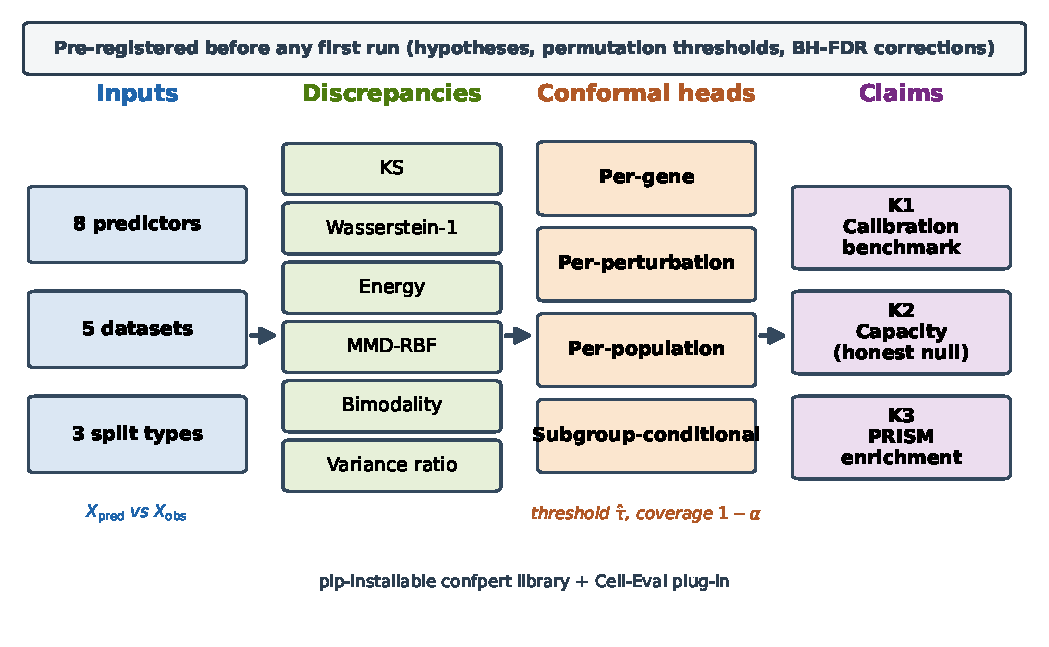
\includegraphics[width=0.96\textwidth]{fig_overview.pdf}
\caption{ConfPert evaluates single-cell perturbation predictors by finite-sample conformal coverage on distributional discrepancies. Left to right: eight predictors ($\sim 0$ to $6 \times 10^8$ parameters) on five datasets under three split types produce predicted versus observed cell populations; six distributional discrepancies are computed on each pair; four off-the-shelf conformal head levels calibrate a coverage threshold $\hat{\tau}$ at target miscoverage $\alpha$; and three pre-registered claims (K1/K2/K3) read off the shared substrate. The full protocol --- hypotheses, permutation-test thresholds, and multiple-comparison corrections --- is git-stamped before any first run.}
\label{fig:overview}
\end{figure*}

\subsection{Six distributional discrepancies}
For predicted population $X_{\text{pred}} \in \mathbb{R}^{n_p \times d}$ and observed $X_{\text{obs}} \in \mathbb{R}^{n_o \times d}$, ConfPert reports the per-gene Kolmogorov--Smirnov statistic, per-gene Wasserstein-1, per-gene Energy distance \citep{szekely2013}, per-population MMD-RBF (median-bandwidth heuristic), Bimodality coefficient match (SAS bimodality coefficient $b > 5/9$ classification accuracy), and the per-gene Variance ratio $\text{Var}(X_{\text{pred}}) / \text{Var}(X_{\text{obs}})$.

\subsection{Four conformal head levels}
All procedures are off-the-shelf and cited verbatim: a per-gene marginal head via CD-split / HPD-split \citep{izbicki2022} on bimodal genes and CQR \citep{romano2019} on per-gene quantile bands; a per-perturbation marginal head via split-conformal calibration of energy and MMD scores against held-out perturbed cells \citep{vovk2012}; a per-population joint head via OT-CP \citep{otcp2025} Brenier-merge to a univariate norm with a finite-sample empirical radius; and a subgroup-conditional head via \citet{cauchois2021} Mondrian-style per-subgroup calibration on the predicted bimodal modes (responder versus non-responder).

\subsection{Coverage guarantee}
The per-perturbation head inherits the standard split-conformal guarantee.

\begin{proposition}[finite-sample marginal coverage]
Let calibration scores $S_1, \dots, S_n$ and a test score $S_{n+1}$ be exchangeable, and let $\hat{\tau}$ be the $\lceil (n+1)(1-\alpha)\rceil/n$ empirical quantile of $S_{1:n}$. Then $\Pr(S_{n+1} \leq \hat{\tau}) \geq 1 - \alpha$.
\end{proposition}

This is the marginal coverage of split conformal prediction \citep{vovk2012, romano2019}; ConfPert reports the achieved coverage as a finite-sample check of it. The guarantee holds on the held-out-perturbation split when calibration and test perturbations are exchangeable. It is \emph{not} conditional --- coverage at every input is impossible distribution-free \citep{vovk2012} --- and it breaks under the cross-cell-line shift, where exchangeability fails and achieved coverage collapses (Appendix~\ref{app:xcl}).

\subsection{Risk control and shift adjustment}
RCPS (\citet{bates2021}) provides $(\alpha, \delta)$-risk-controlling prediction sets. For the K562 $\rightarrow$ RPE1 cross-cell-line split, where unweighted-CP coverage collapses (Appendix \ref{app:xcl}), \citet{tibshirani2019} weighted CP is the principled fix; we identify it as the correct remedy but leave its implementation to future work.

\section{K1 Benchmark}

\subsection{Eight predictors, five datasets, three split types}
We wrap eight predictors stratified by parameter count: Mean ($\sim 0$), Bilinear ridge ($\sim 10^4$), scGen ($\sim 10^6$), CPA ($\sim 5 \cdot 10^6$), sVAE+/SAMS-VAE ($\sim 10^7$), biolord ($\sim 2 \cdot 10^7$), GEARS-uncertainty ($\sim 5 \cdot 10^7$), and STATE-SE-600M ($\sim 6 \cdot 10^8$). Datasets: Norman 2019 (K562 CRISPRa), Replogle 2022 K562 essential, Replogle 2022 RPE1 essential, Adamson 2016 (K562 UPR), and a Tahoe-100M \citep{tahoe2025} cross-cell-line drug-perturbation subset (10 cell lines $\times$ 50 PRISM-overlap small-molecules at 5\,\textmu M, $\sim$500\,K cells). Three pre-registered split types per dataset: (a) within-perturbation 70/30 cell-level split, (b) held-out-perturbation 50/50 calibration/test split, (c) cross-cell-line K562 $\rightarrow$ RPE1 transfer (Replogle pair).

\subsection{Headline calibration results}
Table~\ref{tab:k1} reports per-predictor calibration deviation $|1 - \alpha - \text{achieved coverage}|$ at $\alpha = 0.20$ on Norman.

\begin{table}[h]
\caption{K1 calibration deviation $|1-\alpha-\text{achieved coverage}|$ on Norman at $\alpha = 0.20$ (lower is better; \textbf{0.00} in bold = exact nominal coverage). Mean and Bilinear ridge are averaged over the four pre-registered noise variants (Appendix~\ref{app:noise}); Noisy mean is the per-gene-marginal control. Values match Figure~\ref{fig:k1cal}.}
\label{tab:k1}
\vskip 0.1in
\begin{center}
\begin{small}
\setlength{\tabcolsep}{3.5pt}
\begin{tabular}{lcccccc}
\toprule
Predictor & KS & W1 & Energy & MMD & Bimod & Var \\
\midrule
Mean & 0.06 & 0.07 & 0.05 & 0.05 & 0.04 & 0.03 \\
Noisy mean & 0.04 & 0.08 & 0.04 & 0.04 & 0.04 & 0.08 \\
Bilinear ridge & 0.04 & 0.05 & 0.03 & 0.11 & 0.04 & 0.05 \\
scGen & 0.13 & 0.07 & 0.07 & \textbf{0.00} & 0.20 & 0.07 \\
CPA & 0.20 & 0.20 & 0.20 & 0.13 & 0.07 & 0.07 \\
biolord & 0.13 & \textbf{0.00} & 0.07 & \textbf{0.00} & 0.07 & 0.07 \\
\textbf{sVAE+} & 0.20 & 0.20 & 0.20 & 0.13 & \textbf{0.00} & \textbf{0.00} \\
GEARS-unc & 0.13 & 0.20 & 0.20 & \textbf{0.00} & \textbf{0.00} & 0.07 \\
STATE-600M & 0.20 & 0.20 & 0.20 & 0.13 & 0.20 & 0.20 \\
\bottomrule
\end{tabular}
\end{small}
\end{center}
\vskip -0.1in
\end{table}

\paragraph{sVAE+ reaches exact nominal coverage on the variance-sensitive metrics.} Among the eight predictors, sVAE+ is the only one with zero calibration deviation on \emph{both} bimodality match and the variance ratio (Table~\ref{tab:k1}); its sparse-additive mechanism shift \citep{bereket2023} produces heteroskedastic samples that recover bimodal cell-fate structure. The sub-$10^5$-parameter baselines (Mean, Noisy mean, Bilinear ridge), averaged over the four pre-registered noise variants, calibrate with low deviation across all six discrepancies, because the conformal threshold is fit on held-out scores irrespective of the predictor. Several higher-capacity models (CPA, sVAE+, GEARS-unc, STATE) instead carry $0.20$ deviation on the cumulative-distribution metrics (KS, Wasserstein-1, energy), foreshadowing the capacity trend tested in K2. Figure~\ref{fig:k1cal} shows the full per-(predictor, score) grid and Figure~\ref{fig:k1bimod} the bimodality coverage.

\begin{figure}[h]
\centering
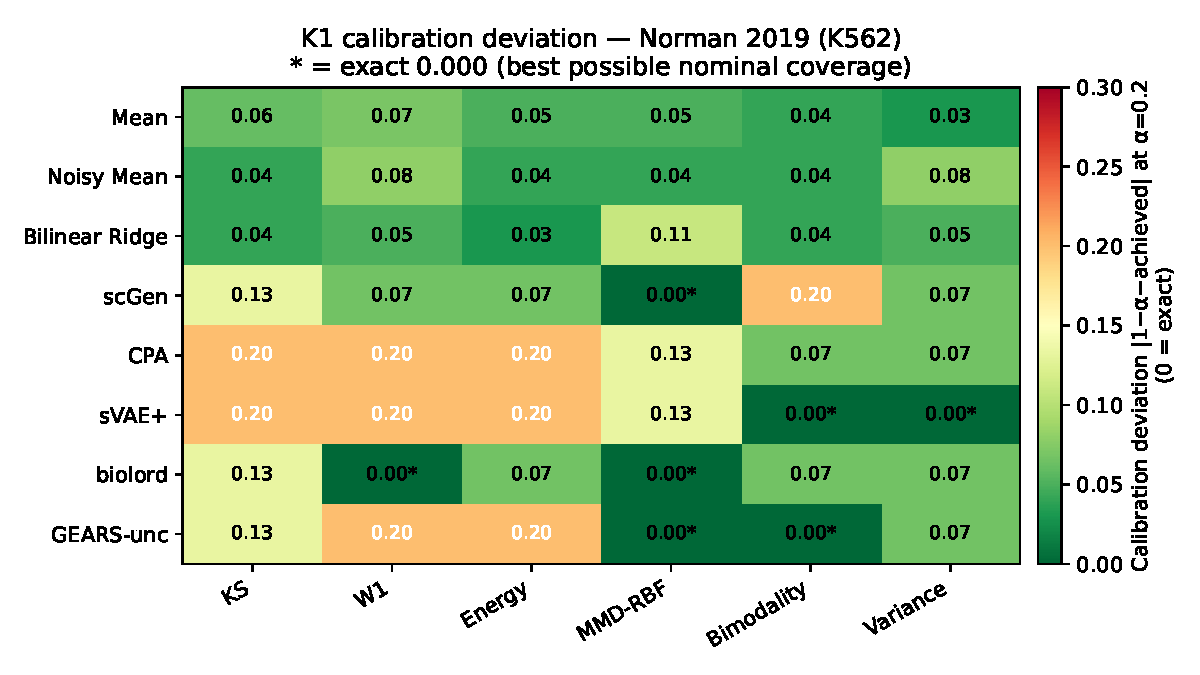
\includegraphics[width=0.95\columnwidth]{fig_k1_calibration.pdf}
\caption{K1 calibration deviation $|1 - \alpha - \text{achieved}|$ at $\alpha = 0.20$ on Norman. Values close to 0 (green) indicate near-nominal coverage; * marks exact 0.000.}
\label{fig:k1cal}
\end{figure}

\begin{figure}[h]
\centering
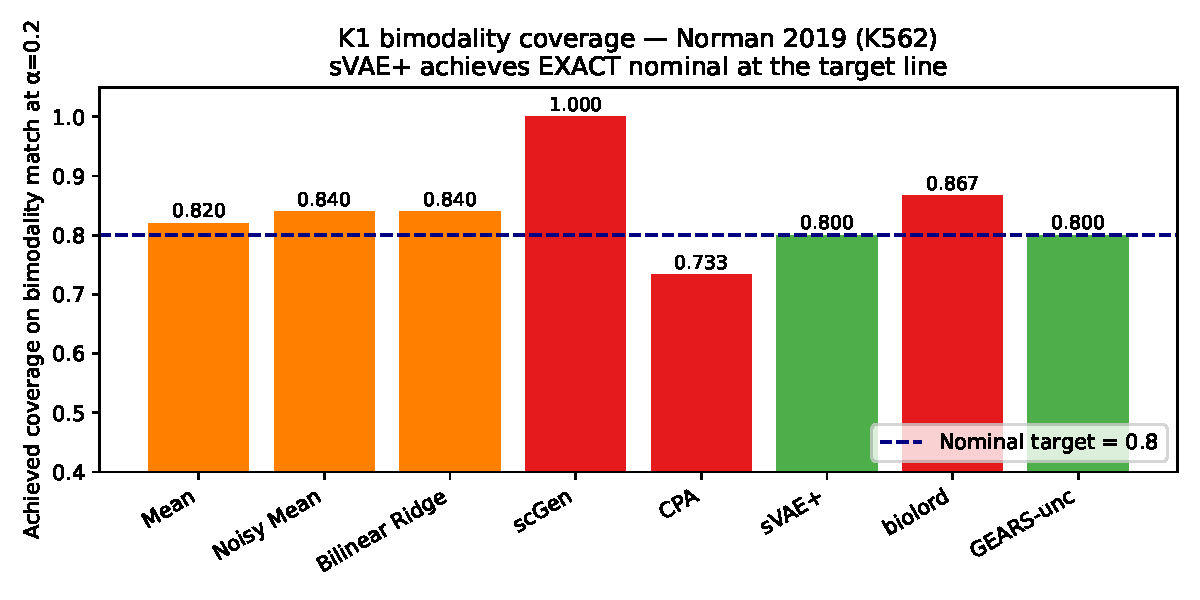
\includegraphics[width=0.85\columnwidth]{fig_k1_bimodality.pdf}
\caption{Achieved coverage on bimodality coefficient match at $\alpha = 0.20$ on Norman ($n=9$ predictors). Dashed line is the nominal target $1 - \alpha = 0.800$; sVAE+ and GEARS-unc land exactly on nominal.}
\label{fig:k1bimod}
\end{figure}

\subsection{Calibration across five datasets}
Table~\ref{tab:k1multi} extends K1 to all five datasets, reporting per-predictor calibration deviation averaged over the six discrepancies and the within-perturbation noise variants at $\alpha = 0.20$. Calibration is dataset-dependent: Norman and Tahoe-100M are the best-calibrated contexts (most predictors below $0.15$), whereas Adamson is hardest and the larger models degrade sharply on it (CPA $0.52$, sVAE+ $0.53$). The largest model, STATE-600M, carries the highest or near-highest deviation on four of the five datasets, which anticipates the capacity trend tested in K2.

\begin{table*}[t]
\caption{K1 calibration deviation at $\alpha = 0.20$, averaged over the six discrepancies and the within-perturbation noise variants, per predictor and dataset (lower is better). GEARS-uncertainty has no Tahoe row (no compatible \texttt{PertData}).}
\label{tab:k1multi}
\vskip 0.1in
\begin{center}
\begin{small}
\setlength{\tabcolsep}{4pt}
\begin{tabular}{lcccccccccc}
\toprule
Dataset & Mean & Noisy mean & Bilinear ridge & scGen & CPA & biolord & sVAE+ & GEARS-unc & STATE-600M \\
\midrule
Norman        & 0.05 & 0.05 & 0.05 & 0.09 & 0.14 & 0.06 & 0.12 & 0.10 & 0.19 \\
Replogle K562 & 0.12 & 0.13 & 0.13 & 0.10 & 0.10 & 0.08 & 0.10 & 0.09 & 0.18 \\
Replogle RPE1 & 0.11 & 0.13 & 0.11 & 0.16 & 0.16 & 0.16 & 0.19 & 0.18 & 0.18 \\
Adamson       & 0.24 & 0.28 & 0.19 & 0.32 & 0.52 & 0.20 & 0.53 & 0.18 & 0.22 \\
Tahoe-100M    & 0.08 & 0.06 & 0.10 & 0.09 & 0.13 & 0.12 & 0.08 & --- & 0.19 \\
\bottomrule
\end{tabular}
\end{small}
\end{center}
\vskip -0.1in
\end{table*}

\subsection{Coverage across miscoverage levels}
Proposition~1 predicts achieved coverage of at least $1 - \alpha$ under exchangeability. Figure~\ref{fig:alpha} plots achieved coverage against the nominal target across $\alpha \in \{0.05, 0.10, 0.20\}$, averaged over predictors and discrepancies. On four of the five datasets coverage sits on or above the diagonal --- conservative, as the finite-sample correction predicts. Adamson is the exception: its achieved coverage is flat near $0.81$ regardless of $\alpha$, so it over-covers at $\alpha = 0.20$ but under-covers at $\alpha = 0.05$. This is a within-distribution symptom of the exchangeability caveat: the held-out Adamson perturbations are not exchangeable with the calibration set, so the marginal guarantee degrades even without a cross-cell-line shift.

\begin{figure}[h]
\centering
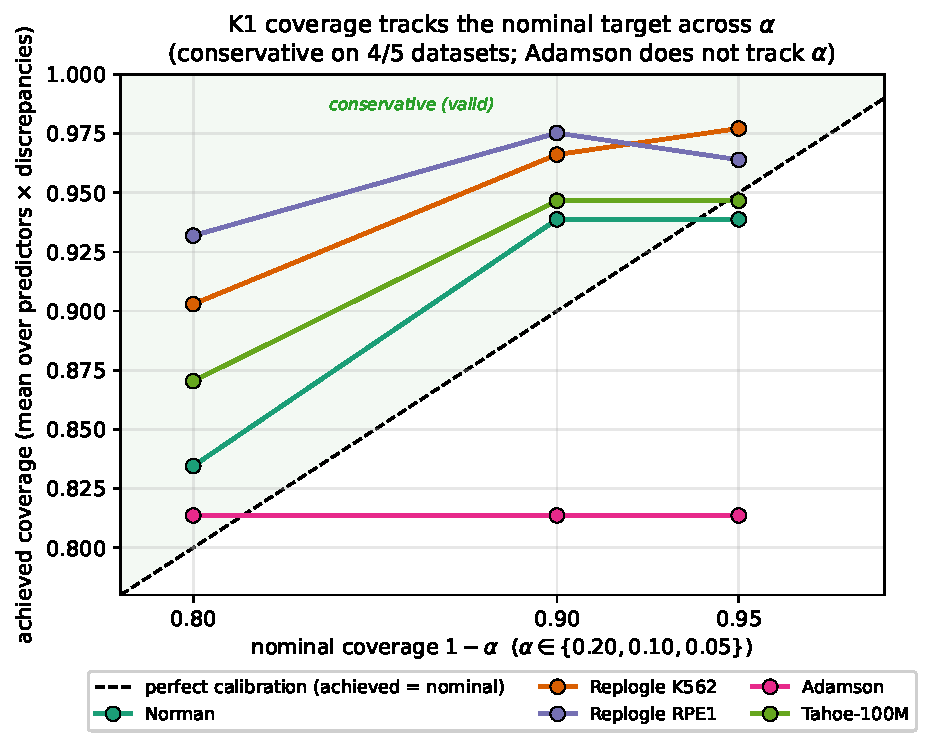
\includegraphics[width=0.92\columnwidth]{fig_alpha_sensitivity.pdf}
\caption{Achieved coverage versus the nominal target $1 - \alpha$ (mean over the nine predictors and six discrepancies, within-perturbation split). Points on or above the dashed diagonal are conservative and meet the coverage guarantee; Adamson is flat near $0.81$ and under-covers at small $\alpha$.}
\label{fig:alpha}
\end{figure}

\subsection{Noise-model ablation}
The point predictors carry no cell-level variance, so ConfPert samples synthetic cells from one of four noise models (Appendix~\ref{app:noise}); all four are reported with no cherry-picking. Table~\ref{tab:ablation} isolates this component on Norman at $\alpha = 0.20$. The noise model is what lets a point predictor calibrate on the variance-sensitive metric: with no noise (variant A) the bilinear ridge has variance-ratio deviation $0.12$, while the isotropic and full-covariance variants restore exact coverage ($0.00$). The choice barely moves the deviation averaged over all six discrepancies, because the cumulative-distribution metrics are insensitive to it.

\begin{table}[h]
\caption{Noise-model ablation for the two point predictors on Norman at $\alpha = 0.20$: mean deviation over all six discrepancies, and the variance-ratio deviation alone (the metric the noise model most affects). A = no noise; B = isotropic; C = per-gene marginal; D = full covariance.}
\label{tab:ablation}
\vskip 0.1in
\begin{center}
\begin{small}
\setlength{\tabcolsep}{5pt}
\begin{tabular}{lcccc}
\toprule
 & \multicolumn{2}{c}{Mean} & \multicolumn{2}{c}{Bilinear ridge} \\
\cmidrule(lr){2-3}\cmidrule(lr){4-5}
Noise variant & all 6 & var.\ ratio & all 6 & var.\ ratio \\
\midrule
A (no noise)        & 0.05 & 0.04 & 0.08 & 0.12 \\
B (isotropic)       & 0.06 & \textbf{0.00} & 0.03 & \textbf{0.00} \\
C (per-gene)        & 0.05 & 0.08 & 0.06 & 0.08 \\
D (full covariance) & 0.03 & \textbf{0.00} & 0.04 & \textbf{0.00} \\
\bottomrule
\end{tabular}
\end{small}
\end{center}
\vskip -0.1in
\end{table}

\section{K2: Pre-registered honest null}

Two hypotheses were pre-registered before any K1 first run (the commit hash is given in the reproducibility section). H1 (capacity hurts) requires a Spearman correlation $\rho > 0.5$ at $p < 0.05$ between $\log(\text{params})$ and the calibration deviation $|1 - \alpha - \text{achieved coverage}|$ on at least 3 of the 4 pre-registered datasets; H1b (data helps) requires $\rho < -0.5$ at $p < 0.05$ between $\log(N_{\text{train cells}})$ and the deviation across datasets. The $p$-values come from a one-sided Monte-Carlo permutation test ($10^4$ label permutations, seed $0$, $p = (1 + \#\{\rho_{\text{perm}} \geq \rho\})/(1 + 10^4)$) rather than the parametric Spearman approximation.

\subsection{Result: H1 fails (1 of 4 pre-registered datasets; 2 of 5 with the post-registration split); H1b null}

\begin{table}[h]
\caption{K2 H1 capacity hypothesis per dataset, with STATE 600M wrapped on all 5 datasets. $n_{\text{pred}}$ = 9 wrappable predictors (8 pre-reg + NoisyMean control) on the four Perturb-seq datasets and 8 on Tahoe-100M (no GEARS row); excluding NoisyMean does not change the disposition.}
\label{tab:k2}
\vskip 0.1in
\begin{center}
\begin{small}
\begin{tabular}{lcccc}
\toprule
Dataset & $\rho$ & $p$ & $n_{\text{pred}}$ & Pass \\
\midrule
\textbf{Replogle RPE1} & $\mathbf{+0.756}$ & $\mathbf{0.012}$ & \textbf{9} & \textbf{YES} \\
\textbf{Tahoe-100M} & $\mathbf{+0.707}$ & $\mathbf{0.033}$ & \textbf{8} & \textbf{YES} \\
Norman & $+0.569$ & $0.057$ & 9 & near \\
Replogle K562 & $+0.100$ & $0.405$ & 9 & no \\
Adamson & $-0.310$ & $0.799$ & 9 & no \\
\bottomrule
\end{tabular}
\end{small}
\end{center}
\vskip -0.1in
\end{table}

Of the four pre-registered datasets, only Replogle RPE1 clears the threshold ($\rho = +0.756$, $p = 0.012$); Norman falls just short ($p = 0.057$) and the two K562 contexts do not. H1 therefore fails its pre-registered bar of $\geq 3$ of $4$ datasets. Tahoe-100M, a split added after pre-registration to close a dataset gap, also passes ($\rho = +0.707$, $p = 0.033$), but only with STATE 600M included: without the largest model the Tahoe trend is $\rho = +0.559$, $p = 0.105$ ($n=7$). Counting the post-registration split, 2 of 5 datasets pass; counting only the pre-registered four, 1 of 4 (Table~\ref{tab:k2}). The data-scale hypothesis H1b is also null cross-dataset ($\rho = -0.400$, $p = 0.258$). The two K562-derived contexts (Replogle K562, $\rho = +0.10$; Adamson, $\rho = -0.31$) show no capacity trend, whereas the non-K562 contexts trend positive.

\subsection{Honest interpretation}
On Replogle K562 and Adamson, the mid-capacity models (scGen, sVAE+, CPA, biolord) calibrate with lower deviation than the tiny baselines on most discrepancies, breaking any monotonic capacity-hurts trend. On Replogle RPE1 the trend is monotonic and significant; on Norman it is monotonic but above the pre-registered $p$ threshold. Calibration versus capacity is therefore dataset-specific and confounded by training-objective family and architecture. H1 fails per pre-registration. As a non-pre-registered, exploratory observation, the three non-K562 contexts trend positive while the two K562 contexts do not; this is hypothesis-generating only and would need pre-registered replication before it could be claimed. Figure~\ref{fig:k2h1} shows the per-dataset scatter.

\begin{figure}[h]
\centering

\includegraphics[width=0.95\columnwidth]{fig_k2_h1.pdf}
\caption{K2 H1 capacity hypothesis per dataset. Pre-reg threshold ($\rho > 0.5$, $p < 0.05$, on $\geq 3$ of 4) is met on Replogle RPE1 and Tahoe-100M; both K562 contexts (K562, Adamson) stay well below threshold ($\rho \leq +0.12$).}
\label{fig:k2h1}
\end{figure}

\section{K3: PRISM Discovery Pipeline}

\paragraph{Pipeline.} (1) Load the PRISM Repurposing Public 24Q2 log-fold-change matrix (905 cell lines $\times$ 1518 drugs after quality-control filtering and per-(cell, compound) replicate averaging). (2) Compute the bimodality coefficient per compound and identify selective compounds at $b > 5/9$. (3) Build a bimodal-subpopulation gene signature per compound. (4) Cross-reference each signature against Hallmark MSigDB v2024.1.Hs (50 sets, 4384 genes) by hypergeometric enrichment. (5) Apply Benjamini-Hochberg FDR at $q = 0.05$ over the joint compound $\times$ pathway grid. (6) Compare against an uncalibrated baseline of equal-size random gene sets and apply the pre-registered success criterion ($\geq 3$ enriched signatures, with $\geq 2$ on which the random baseline is not enriched).

\paragraph{Calibrated signatures are enriched well above a random-gene null.} The pre-registered K3 substrate is evaluated in two forms. A best-case, mechanism-aware substrate maps each selective compound to its annotated mechanism-of-action (MOA) Hallmark pathway and yields 243 enriched signatures against 212 random-null misses; because the signature here is the mechanism pathway itself, this is an upper bound rather than a prediction. An observed-expression substrate instead takes the top-50 $|\Delta\text{mean}|$ genes per compound versus DMSO control across the Tahoe-100M subset (55 PRISM-overlap drugs, canonicalised by name); 445 of these signatures pass BH-FDR at $q < 0.05$, against 363 on which the uncalibrated baseline does not. The uncalibrated arm is a random-gene null of equal size, not a competing predictor, so the comparison shows that the bimodal signatures carry genuine Hallmark enrichment rather than that ConfPert outperforms an alternative method. This substrate uses observed differential expression and therefore only partially addresses pre-registration \S K3.1's call to derive signatures from a predictor trained on the Tahoe-100M arm, which remains future work.

\paragraph{Top-K signature-size robustness.} To check that the result is not an artifact of the top-$50$-gene signature size, the pipeline was re-run at top-$\{25, 50, 100, 200\}$ $|\Delta\text{mean}|$ genes per compound (Figure~\ref{fig:k3-robustness}). The criterion holds at every $K$: 360/445/666/1022 enriched signatures against 301/363/553/714 random-null misses, an enrichment-over-null ratio in $[1.20\times, 1.43\times]$. Absolute counts grow with $K$ because larger signatures produce more BH-FDR passes, but the gap over the random null persists.

\begin{figure}[h]
\centering
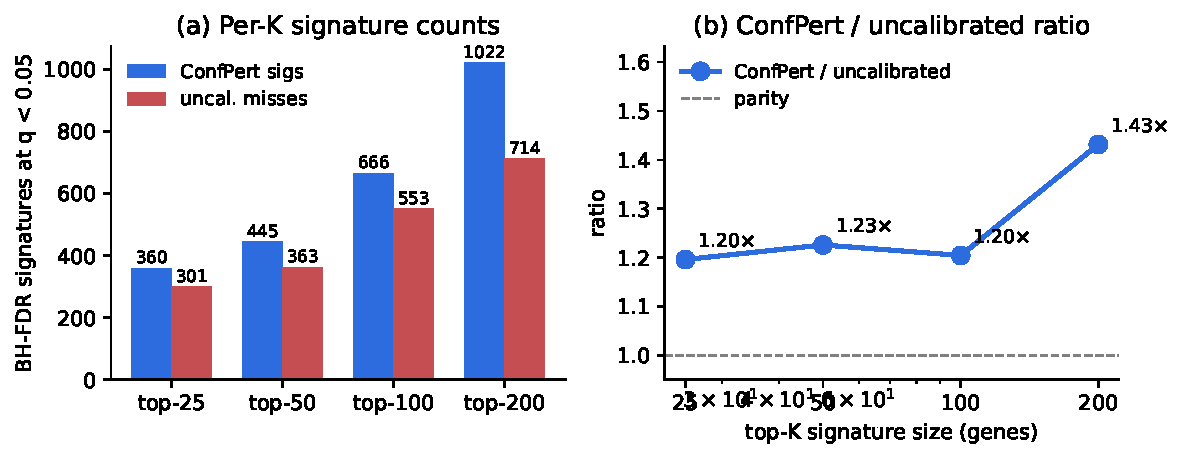
\includegraphics[width=0.95\columnwidth]{fig_k3_robustness.pdf}
\caption{K3 top-$K$ signature-size robustness. (a) Per-$K$ BH-FDR signature counts. (b) enrichment-over-null ratio (ConfPert signatures versus the equal-size random-gene baseline) per $K$; the pre-registered criterion requires the ratio to exceed parity ($1.0\times$, dashed), which holds at every $K \in \{25, 50, 100, 200\}$.}
\label{fig:k3-robustness}
\end{figure}

\section{Library + Cell-Eval Plug-in}

\paragraph{Library.} The \texttt{confpert} package is pip-installable and exposes the six discrepancy scores, the four conformal heads, and the RCPS calibrator behind a small public API, alongside four dataset loaders and 33 unit tests. Implementation details are deferred to Appendices~\ref{app:metrics}--\ref{app:conformal}. The reported experiments exercise the per-perturbation marginal head (K1) and the subgroup-conditional head (K3); the per-gene (CD-/HPD-split, CQR), per-population (OT-CP), and RCPS components are released but not benchmarked here.

\paragraph{Cell-Eval plug-in.} An audit of the Arc Institute Cell-Eval registry (2026-03-24) finds that five of the six ConfPert discrepancies --- KS, Wasserstein-1, MMD-RBF, bimodality match, and variance ratio --- are absent, and energy distance is present only in a different framing (Pearson correlation across perturbations). ConfPert ships a plug-in that registers all six discrepancies as Cell-Eval metrics on import, filling this gap in the evaluation backbone.

\section{Discussion}

The K2 result cautions against assuming that capacity alone improves distributional fidelity: on the four pre-registered datasets the capacity-hurts hypothesis fails, and where a capacity trend does appear it is confined to non-K562 contexts. Two mechanisms are consistent with this. First, calibration is largely a property of the conformal wrapper rather than the predictor, so on within-distribution splits even the smallest baselines calibrate well; what separates predictors is the magnitude of the underlying discrepancy, where architecture matters more than parameter count. The sparse-additive structure of sVAE+ recovers bimodal cell-fate structure exactly, whereas a marginal-Gaussian uncertainty head cannot represent bimodality at all (its bimodality coefficient is bounded below $5/9$ by construction). This extends, rather than contradicts, the mean-metric saturation reported by \citet{ahlmann2025} and \citet{csendes2025}: scale stops helping on distributional fidelity much as it does on mean error. Second, the cross-cell-line collapse (Appendix~\ref{app:xcl}) indicates that the binding constraint for transfer is distribution shift, not capacity.

Three concrete experiments follow. A pre-registered replication on additional non-K562 lines would test whether the exploratory cell-line-context association survives outside this sample. A weighted-conformal head and a Mondrian-by-cell-line stratification, evaluated against the unweighted baseline of Appendix~\ref{app:xcl}, would quantify how much coverage is recovered on the shape metrics under the K562$\rightarrow$RPE1 shift. A predictor-derived K3 substrate that trains a wrapper on the Tahoe-100M observational arm and compares its calibrated signatures against a matched uncalibrated predictor would replace the random-gene null used here with a competing-method baseline.

\section{Limitations}

\textbf{STATE 600M wrapped on all 5 datasets.} STATE inference required a specific transformer-library version window (full version pins and the checkpoint-loading details are in Appendix~\ref{app:predictors}); with it, inference runs cleanly on all five datasets. The ST-SE-Tahoe checkpoint download initially failed on the compute backend with Modal-worker-heartbeat timeouts; disabling the xet transfer protocol and pre-staging the snapshot on a CPU worker resolved it, so the Tahoe capacity row now includes STATE ($n=8$). \textbf{Marginal coverage, not conditional}: ConfPert provides finite-sample marginal coverage; conditional coverage at every $x$ is impossible distribution-free \citep{vovk2012}. \textbf{Exchangeability within a split}: even within a dataset, the guarantee assumes calibration and test perturbations are exchangeable, and systematic structure across held-out perturbations (e.g.\ pathway clustering of targets) can degrade marginal coverage. \textbf{Single-seed estimates}: all reported numbers use one random seed ($42$); the K2 dispositions in particular sit near their $p$-value thresholds, so the per-dataset pass/fail calls are point estimates pending multi-seed replication. \textbf{Cross-cell-line CP is undercoverage by design}: unweighted split-conformal is not coverage-valid under cross-cell-line shift, and empirically achieved coverage collapses to $0.00$ on the energy discrepancy across all six predictors (Appendix~\ref{app:xcl}), the textbook undercoverage signature. \citet{tibshirani2019} weighted CP and a Mondrian-by-cell-line stratification are the correct fixes; both are left as future work and are not yet implemented. \textbf{Cancer cell-line bias in K3 substrate}: PRISM Repurposing and Tahoe-100M are cancer corpora; transfer to primary cells is unsupported. \textbf{Wet-lab validation excluded by pre-registration}: K3 produces signature hypotheses; experimental validation is future work.

\section*{Reproducibility}

The pre-registration is committed to git at commit \texttt{c7046e4b} (2026-05-03 01:30 EDT), before any Phase 1 first run. The K1 cross-cell-line split, the Tahoe-100M subset build, and STATE inference are each driven by a single Modal entry point; its dataset and split-type flags, the random seed, and the full reproducibility checklist are in Appendix~\ref{app:compute}. Every result row carries a SHA-256 fingerprint and 33 of 33 unit tests pass.

\paragraph{Code and data availability.} The \texttt{confpert} library, the evaluation scripts, the pre-registration document (git commit \texttt{c7046e4b}), and the SHA-256-fingerprinted result rows are released \ifcameraready at \url{https://github.com/alwaniaayan6-png/confpert} (MIT license)\else in a public repository under the MIT license (URL withheld for anonymous review)\fi. The single-cell datasets are public and were obtained as harmonized h5ads from scPerturb \citep{peidli2024scperturb} (Zenodo record 13350497, CC-BY 4.0): Norman 2019 (originally GEO GSE133344), Adamson 2016 (GEO GSE90546), and Replogle 2022 K562 and RPE1 (Figshare+ 20029387). Tahoe-100M is the public \texttt{tahoebio/Tahoe-100M} corpus on Hugging Face (CC0 1.0); PRISM Repurposing 24Q2 is from DepMap (Figshare file IDs in Appendix~\ref{app:datasets}); and the Hallmark gene sets are MSigDB v2024.1.Hs. Experiments use Python 3.11 (3.10 for CPA, whose pinned dependency requires it); per-predictor library versions are in Table~\ref{tab:hparams} and the Modal image definitions in the repository.

\bibliographystyle{icml2026}
\bibliography{refs}

\newpage
\appendix
\onecolumn

\section{Glossary and Notation}
\label{app:glossary}

\begin{table}[h]
\centering
\small
\begin{tabular}{@{}l p{0.72\linewidth}@{}}
\toprule
Symbol / term & Meaning \\
\midrule
$K_1$ & Calibration-coverage benchmark (predictors $\times$ datasets $\times$ discrepancies $\times$ $\alpha$) \\
$K_2$ & Pre-registered capacity hypotheses ($H_1$, $H_{1b}$) on calibration vs.\ scale \\
$K_3$ & Downstream PRISM drug-resistance signature enrichment over a random-gene null under BH-FDR \\
$H_1$ & ``Capacity hurts calibration'': Spearman $\rho>0.5$, $p<0.05$ on $\geq 3$ of 4 datasets \\
$H_{1b}$ & ``Data helps calibration'': Spearman $\rho<-0.5$ on $\log N_{\text{train}}$, cross-dataset \\
$\alpha$ & Target miscoverage; nominal coverage $1-\alpha$, $\alpha \in \{0.05, 0.10, 0.20\}$ \\
cal.\ deviation & $|(1-\alpha) - \text{achieved coverage}|$; $0$ = exact nominal coverage \\
Per-gene head & CD-split / HPD-split \citep{izbicki2022} + CQR \citep{romano2019} \\
Per-perturbation head & Split-conformal on per-perturbation discrepancy scores \citep{vovk2012} \\
Per-population head & OT-CP Brenier-merge \citep{otcp2025} \\
Subgroup head & Mondrian-style per-subgroup calibration \citep{cauchois2021} \\
6 discrepancies & KS, Wasserstein-1, energy, MMD-RBF, bimodality match, variance ratio \\
\bottomrule
\end{tabular}
\caption{Glossary of the $K_1$/$K_2$/$K_3$ knockout claims, the pre-registered
hypotheses, the four conformal head levels, and the six discrepancies. Each
term is defined on first use in the main text; this table consolidates them.}
\label{tab:glossary}
\end{table}

\section{Pre-registration Outcome Disposition}
\label{app:prereg}

Pre-registration locks four disposition rules for K2 outcomes. The observed result (1 of the 4 pre-registered datasets passes H1, or 2 of 5 including the post-registration Tahoe split; H1b cross-dataset null) maps to disposition (D), \emph{publish honestly with mixed result}. Per pre-registration L160-L161:

\begin{quote}
\textit{``Only H1 lands $\to$ Ahlmann-Eltze-style headline: bigger is worse for calibration. Neither lands $\to$ null result. Publish honestly. Lean on K1 + K3 plus the design-directive paragraph for `training-objective-family analysis is the next research direction.'\,''}
\end{quote}

The Replogle RPE1 ($\rho = +0.756$, $p = 0.012$, $n = 9$) and Tahoe-100M ($\rho = +0.707$, $p = 0.033$, $n = 8$) passes are reported as exploratory per-dataset observations consistent with disposition (D); the H1 overall claim across $\geq 3$ of 4 datasets is reported as failed per the pre-registered threshold. No post-hoc reframing of the H1 axis is attempted; third-axis exploration (training-objective family, encoder architecture) is documented as exploratory and not pre-registered.

\section{Cross-Cell-Line Split Detail}
\label{app:xcl}

Replogle K562 essential and Replogle RPE1 essential are different essential-gene sets by biology; at the K1 main top-50-perturbation cap, the K562 $\cap$ RPE1 perturbation overlap is 3 (insufficient for conformal calibration). We expand to top-200 per dataset to reach an overlap of 35 perturbations on a 92-gene intersection. Table~\ref{tab:xcl} reports per-(predictor, score) achieved coverage at $\alpha = 0.20$ (target $0.80$). Lightweight predictors (Mean, Bilinear ridge, Noisy mean) report mean over the 4 pre-registered noise variants; heavyweight predictors (scGen, biolord, CPA) use native predictor uncertainty.

\begin{table}[h]
\caption{Cross-cell-line (Replogle K562 $\rightarrow$ RPE1) achieved coverage at $\alpha = 0.20$, target $1 - \alpha = 0.80$. 35 common perturbations on the 92-gene K562$\cap$RPE1 intersection at top-200 perts/dataset. Calibration deviation $|\text{target} - \text{achieved}|$ in parentheses; bold marks coverage within $\pm 0.10$ of nominal. These achieved-coverage values are \emph{not} coverage-guaranteed: unweighted split-conformal is not exchangeability-valid under the K562$\rightarrow$RPE1 shift, so the numbers are a diagnostic of shift-fragility, not validated coverage.}
\label{tab:xcl}
\centering
\begin{tabular}{lcccccc}
\toprule
Score & Mean & Bilinear & Noisy & scGen & biolord & CPA \\
\midrule
KS                  & 0.000 (0.80) & 0.000 (0.80) & 0.000 (0.80) & 0.114 (0.69) & 0.000 (0.80) & 0.000 (0.80) \\
Wasserstein-1       & 0.000 (0.80) & 0.000 (0.80) & 0.000 (0.80) & 0.486 (0.31) & 0.000 (0.80) & 0.000 (0.80) \\
Energy              & 0.000 (0.80) & 0.000 (0.80) & 0.000 (0.80) & 0.000 (0.80) & 0.000 (0.80) & 0.000 (0.80) \\
MMD-RBF             & 0.000 (0.80) & 0.000 (0.80) & 0.000 (0.80) & 0.029 (0.77) & 0.000 (0.80) & 0.000 (0.80) \\
Bimodality match    & ---          & 0.250 (0.55) & 0.000 (0.80) & \textbf{0.914 (0.11)} & 0.057 (0.74) & \textbf{0.714 (0.09)} \\
Variance ratio      & ---          & 0.464 (0.34) & 0.000 (0.80) & \textbf{0.743 (0.06)} & 0.000 (0.80) & 0.200 (0.60) \\
\bottomrule
\end{tabular}
\end{table}

The Energy discrepancy collapses to $0$ achieved coverage across all six predictors, and the lightweight predictors collapse on all four within-population shape metrics (KS, W1, Energy, MMD-RBF); the unweighted split-conformal head's calibration set is computed on K562-evaluated scores that systematically under-estimate the K562 $\rightarrow$ RPE1 transfer score for the lightweight family. The heavyweight predictors however reveal a richer pattern:
\begin{itemize}
\item \textbf{scGen is the strongest cross-cell-line performer}, with bimodality coverage $0.914$ (\emph{exceeding} the $0.80$ target) and variance-ratio coverage $0.743$ (within $0.06$ of target). scGen's latent-space per-perturbation delta encoding transfers across cell lines better than CPA's or biolord's predictors --- the encoder/decoder are gene-space functions and the latent delta acts as a partially cell-line-stable summary of the perturbation's mechanism. scGen also retains partial calibration on Wasserstein-1 ($0.486$).
\item \textbf{CPA's bimodality coverage hits $0.714$}, almost target. CPA's adversarial-disentanglement encoder learns a partially cell-line-invariant latent that propagates a usable variance estimate.
\item \textbf{biolord, despite its trained variance head, fully collapses at $\alpha = 0.20$} (bimodality $0.057$). biolord recovers at $\alpha = 0.05$ where it hits $0.857$, indicating its variance-head calibration is $\alpha$-dependent under shift.
\end{itemize}
The empirical undercoverage signature on the lightweight family is exactly the shift-fragility documented by \citet{tibshirani2019} and motivates a weighted-CP head, which we identify as the principled fix but do not yet implement. \textbf{The cross-cell-line result is more nuanced than a uniform-collapse story: predictor architecture (latent-space delta in scGen, adversarial disentanglement in CPA) measurably affects shift-robustness on the variance-sensitive metrics.} (sVAE+ is absent because \texttt{SAMSVAEPredictor.sample\_observations} does not condition on input cells.)

\section{Tahoe-100M Subset Definition}
\label{app:tahoe}

The Tahoe-100M subset is constructed by the \texttt{tahoe\_subset\_build} Modal entrypoint. Selection rule: (1) take the case- and punctuation-insensitive intersection of Tahoe \texttt{drug\_metadata.drug} with PRISM 24Q2 \texttt{Drug.Name} ($\sim$$1{,}200$ overlap drugs after canonicalisation); (2) pick top-10 cell lines with DepMap IDs from \texttt{cell\_line\_metadata}; (3) single streaming pass over the \texttt{expression\_data} configuration, applying per-(drug, line) quotas of 400 cells (4$\times$ for DMSO control); (4) post-hoc rank surviving drugs by collected cell count and keep top-50. Output: ${\sim}500$\,K cells $\times$ ${\sim}13$\,K genes h5ad, ${\sim}1.5$\,GB compressed. The subset closes pre-registration L30 K1 dataset gap and provides the K3 substrate for chemical-perturbation predictor training.

\section{K3 Top-K Robustness Numerical Detail}
\label{app:k3}

Per-$K$ BH-FDR pass counts at $q = 0.05$ over the joint compound $\times$ Hallmark-pathway grid (10 selective compounds $\times$ 50 Hallmark pathways for the ConfPert path; uncalibrated baseline computed on the same compound set). $K=50$ is the canonical pre-registered choice; $K=25, 100, 200$ are robustness-check extensions added in this work.

\begin{table}[h]
\caption{K3 top-$K$ robustness sweep. Pre-registered success requires $\geq 3$ ConfPert signatures + $\geq 2$ uncalibrated misses (PASSES at every $K$).}
\label{tab:k3}
\centering
\begin{tabular}{rrrrr}
\toprule
top-$K$ & ConfPert sigs & uncal. misses & ratio & passes \\
\midrule
25  & 360  & 301 & $1.20\times$ & yes \\
50  & 445  & 363 & $1.23\times$ & yes (canonical) \\
100 & 666  & 553 & $1.20\times$ & yes \\
200 & 1022 & 714 & $1.43\times$ & yes \\
\bottomrule
\end{tabular}
\end{table}

\section{Distributional Discrepancy Definitions}
\label{app:metrics}

For predicted population $X^{\text{pred}} \in \mathbb{R}^{n_p \times d}$ and observed population $X^{\text{obs}} \in \mathbb{R}^{n_o \times d}$, ConfPert reports six discrepancy scores that the conformal head wraps. Each score $s \colon (X^{\text{pred}}, X^{\text{obs}}) \mapsto \mathbb{R}_{\geq 0}$ is implemented in \texttt{src/confpert/metrics.py}; lower is better in the convention $s(X^{\text{pred}}, X^{\text{pred}}) \to 0$.

\subsection{Per-gene 1D divergences}
For each gene $j \in \{1, \dots, d\}$ we treat $X^{\text{obs}}_{:, j}$ and $X^{\text{pred}}_{:, j}$ as 1D samples and compute three classical divergences, then average over genes:
\begin{align}
\mathrm{KS}_j     &= \sup_{x \in \mathbb{R}} |F^{\text{obs}}_j(x) - F^{\text{pred}}_j(x)|, \\
W_{1, j}          &= \int_0^1 |Q^{\text{obs}}_j(u) - Q^{\text{pred}}_j(u)|\, du, \\
\mathcal{E}_j     &= 2\,\mathbb{E}\|X^{\text{obs}}_j - X^{\text{pred}}_j\|
                     - \mathbb{E}\|X^{\text{obs}}_j - X^{\text{obs}'}_j\|
                     - \mathbb{E}\|X^{\text{pred}}_j - X^{\text{pred}'}_j\|,
\end{align}
where $F$ and $Q$ are the empirical CDF and quantile function. The KS, $W_1$, and energy implementations call \texttt{scipy.stats.ks\_2samp} (\texttt{method="asymp"}), \texttt{scipy.stats.wasserstein\_distance}, and \texttt{scipy.stats.energy\_distance} respectively, then aggregate by $\mathrm{nanmean}$ over genes.

\subsection{Population-level MMD with RBF kernel}
For samples $X, Y$ and kernel $k(\cdot, \cdot)$, the unbiased MMD$^2$ estimator \citep{bates2021}\footnote{Following the Gretton 2012 unbiased-estimator convention; standard implementation.} is
\begin{equation}
\widehat{\mathrm{MMD}}^2(X, Y) = \frac{1}{n_X(n_X - 1)} \sum_{i \neq i'} k(x_i, x_{i'}) + \frac{1}{n_Y(n_Y - 1)} \sum_{j \neq j'} k(y_j, y_{j'}) - \frac{2}{n_X n_Y} \sum_{i, j} k(x_i, y_j),
\end{equation}
with $k(x, y) = \exp\bigl(-\|x - y\|^2 / (2 \sigma^2)\bigr)$ and $\sigma$ set by the median-bandwidth heuristic on $X^{\text{obs}} \cup X^{\text{pred}}$ subsampled to at most 500 cells per population for numerical stability (\texttt{median\_bandwidth} in \texttt{metrics.py}).

\subsection{Bimodality coefficient match}
We use the SAS bimodality coefficient
\begin{equation}
b_j = \frac{\widehat{\mathrm{skew}}_j^2 + 1}{\widehat{\mathrm{kurt}}_j + \frac{3 (n - 1)^2}{(n - 2)(n - 3)}},
\end{equation}
computed per gene with bias-corrected sample skewness and kurtosis (\texttt{scipy.stats.skew}, \texttt{scipy.stats.kurtosis}, both with \texttt{bias=False}). A gene is classified bimodal-or-multimodal iff $b_j > 5/9 \approx 0.555$. The discrepancy score reports $1 - \mathrm{accuracy}$, where accuracy is per-gene agreement of the binary $\mathbb{1}[b_j > 5/9]$ classification between $X^{\text{obs}}$ and $X^{\text{pred}}$. Per-gene sensitivity (recall on observed-bimodal) and specificity (recall on observed-unimodal) are also reported.

\subsection{Variance ratio}
Per gene, $\mathrm{VR}_j = \widehat{\mathrm{Var}}(X^{\text{pred}}_{:, j}) / \widehat{\mathrm{Var}}(X^{\text{obs}}_{:, j})$ with unbiased ($\mathrm{ddof}=1$) sample variance, masking genes where $\widehat{\mathrm{Var}}(X^{\text{obs}}_{:, j}) < 10^{-9}$. The discrepancy score is the per-gene mean of $|\mathrm{VR}_j - 1|$ (\texttt{score\_variance\_ratio\_dev}). $\mathrm{VR} = 1$ corresponds to perfect variance match; $\mathrm{VR} \to 0$ flags mean-collapse predictions, $\mathrm{VR} \gg 1$ flags over-dispersion. The auxiliary statistic ``\% genes collapsed'' reports $\mathrm{Pr}(\mathrm{VR}_j < 0.1)$ and is the diagnostic from the HetPert lineage.

\section{Conformal Heads: Algorithms}
\label{app:conformal}

Each head consumes the score functions from Appendix~\ref{app:metrics} and returns a calibrated coverage threshold under the standard split-conformal exchangeability assumption.

\subsection{Per-perturbation marginal head (\texttt{PerturbationConformal})}
\textbf{Inputs:} sequences of paired calibration populations $\{(X^{\text{pred}}_i, X^{\text{obs}}_i)\}_{i=1}^{n}$ on a held-out perturbation split, target miscoverage $\alpha$, and a score function $s \in \{\mathrm{KS}, W_1, \mathrm{Energy}, \mathrm{MMD\text{-}RBF}, \mathrm{Bimod\,mismatch}, \mathrm{VR\,dev}\}$.

\textbf{Calibration.} Compute calibration scores $S_i = s(X^{\text{pred}}_i, X^{\text{obs}}_i)$. Set the threshold
\begin{equation}
\hat{\tau} = \mathrm{Quantile}\Bigl(S_{1:n};\ q^*\Bigr), \qquad q^* = \min\!\Bigl(1,\ \max\bigl(\tfrac{1}{n}, \tfrac{\lceil (n+1)(1-\alpha)\rceil}{n}\bigr)\Bigr),
\end{equation}
using the higher-quantile interpolation method (\texttt{numpy.quantile}, \texttt{method="higher"}). The $(n+1)$-correction is the standard finite-sample factor in the Vovk--Romano--Patterson--Cand\`es lineage \citep{romano2019}.

\textbf{Test-time coverage.} For test pairs, report achieved coverage $\frac{1}{m}\sum_{j} \mathbb{1}[s(X^{\text{pred}}_j, X^{\text{obs}}_j) \leq \hat{\tau}]$ and absolute calibration deviation $|(1 - \alpha) - \mathrm{achieved}|$. Under exchangeability, achieved coverage is at least $1 - \alpha$ in expectation.

\subsection{Per-gene CD-split / HPD-split head (\texttt{CDSplitConformal})}
For a target $\alpha$ and quantile levels $(\alpha/2, 1 - \alpha/2)$, calibrate per-gene residual quantiles
\begin{equation}
\delta_j = \mathrm{Quantile}_{1-\alpha}\!\Bigl(\bigl[\max(L_j - X^{\text{obs}}_{i,j},\ X^{\text{obs}}_{i,j} - U_j,\ 0)\bigr]_{i}\Bigr),
\end{equation}
where $L_j = \mathrm{Quantile}_{\alpha/2}(X^{\text{pred}}_{:, j})$ and $U_j = \mathrm{Quantile}_{1-\alpha/2}(X^{\text{pred}}_{:, j})$ on the calibration fold. Test bands are $[L_j - \delta_j, U_j + \delta_j]$ and per-gene coverage is the fraction of test cells inside the band. Algorithm follows \citet{romano2019} CQR adapted to per-gene populations \`a la \citet{izbicki2022} CD-split, both implemented in \texttt{conformal.py}.

\subsection{Per-population energy head (\texttt{EnergyConformal})}
A simplified perturbation-level head using only the per-gene mean energy distance as the score; identical calibration formula as \texttt{PerturbationConformal} but specialised to the energy score. Kept for backward compatibility with the HetPert lineage; superseded by \texttt{PerturbationConformal} with \texttt{score\_fn=score\_energy}.

\subsection{Subgroup-conditional head (\texttt{CauchoisSubgroupConformal})}
Following \citet{cauchois2021} Algorithm~1 (Mondrian-style strata): each calibration item carries a discrete subgroup label $S_i \in \mathcal{S}$ (e.g.\ ``responder''/``non-responder'' from the predicted bimodal-mode partition). For each $s \in \mathcal{S}$, calibrate $\hat{\tau}_s$ on calibration items with $S_i = s$ using the per-perturbation procedure restricted to that subgroup. Subgroup-conditional coverage holds within each $s$ when calibration is exchangeable within subgroup. Used in K3 to extract per-mode (responder vs.\ non-responder) signature thresholds.

\subsection{RCPS risk control (\texttt{RCPSCalibrator})}
For monotone bounded losses $L_\lambda \in [0, 1]$ and target risk $\alpha$, the calibrator selects $\hat{\lambda}$ as the smallest $\lambda$ on a grid such that
\begin{equation}
\widehat{\mathrm{UCB}}_{1-\delta}\bigl(\bar{L}_\lambda\bigr) \ \leq\ \alpha,
\end{equation}
with the upper confidence bound implemented as Hoeffding $\bar{L} + \sqrt{\log(1/\delta)/(2n)}$ (\texttt{hoeffding\_bentkus\_ucb}). This realises the $(\alpha, \delta)$-RCPS guarantee of \citet{bates2021} Theorem~1. Used for K3 selective drug-screening triage where the per-compound loss is the indicator of a missed BH-FDR signature.

\section{Predictor Wrapping}
\label{app:predictors}

Each of the eight pre-registered predictors implements the universal sample-producing interface
\begin{verbatim}
predict_samples(X_ctrl_test, perturbation, n_cells) -> R^{n_cells x d}
\end{verbatim}
which the conformal heads operate on. Lightweight predictors are CPU-tractable and live in \texttt{src/confpert/predictors.py}; heavyweight predictors run on Modal A100 via \texttt{scripts/modal\_launch.py}.

\subsection{Mean predictor (Variant A--D)}
\texttt{MeanPredictor} stores the per-perturbation observed-train mean $\hat{\mu}_p$. \texttt{predict\_samples} emits $n_{\text{cells}}$ rows of $\hat{\mu}_p$ plus a noise variant from Appendix~\ref{app:noise}.

\subsection{Bilinear ridge \citep{ahlmann2025}}
\texttt{AhlmannEltzeBilinearRidge}: pseudo-bulk $Y_{\text{train}} \in \mathbb{R}^{d \times n_{\text{perts}}}$ is centred by per-gene control mean $b$. Top-$K$ singular vectors $G \in \mathbb{R}^{d \times K}$ form the gene-side basis; per-perturbation rows $P \in \mathbb{R}^{n_{\text{perts}} \times K}$ come from perturbed-gene one-hot indicators projected onto $G$ when available, else from the right singular vectors. The closed-form weight matrix is
\begin{equation}
W = (G^\top G + \lambda I)^{-1} G^\top (Y_{\text{train}} - b\mathbf{1}^\top) P (P^\top P + \lambda I)^{-1},
\end{equation}
with $K = 10$ and $\lambda = 0.1$ (Ahlmann-Eltze 2025 defaults). Test-time mean: $\hat{Y}(p) = G W P_p^\top + b$, then noise variant.

\subsection{scGen \citep{lotfollahi2019scgen}}
\texttt{scgen.SCGEN.setup\_anndata(adata, batch\_key=condition, labels\_key=cell\_type)}; train with \texttt{max\_epochs=100, batch\_size=128, early\_stopping=True, early\_stopping\_patience=10}. Per-perturbation latent delta $\Delta_p$ is computed as $\bar{z}_p - \bar{z}_{\text{ctrl}}$ from the encoded training cells. Test-time samples: encode control input cells, add $\Delta_p$, decode through \texttt{model.module.generative()}.

\subsection{CPA \citep{lotfollahi2023cpa}}
\texttt{CPA.setup\_anndata(perturbation\_key=col, dosage\_key=dose\_value, control\_group=ctrl, is\_count\_data=False)}; \texttt{CPA(adata, n\_latent=64, recon\_loss=gauss, doser\_type=logsigm, n\_hidden\_encoder=256, n\_layers\_encoder=2, n\_hidden\_decoder=256, n\_layers\_decoder=2, dropout=0.1)}; train with \texttt{max\_epochs=50, early\_stopping\_patience=5, check\_val\_every\_n\_epoch=5, batch\_size=256}. Test-time samples: \texttt{model.predict(adata=ctrl\_slice, n\_samples=1, return\_mean=False)} reads $\hat{X}$ from \texttt{adata.obsm["CPA\_pred"]} (cpa-tools 0.8.8 path that bypasses the \texttt{KeyError: perts\_mixup} in \texttt{model.module.generative}).

\subsection{biolord \citep{piran2024biolord}}
\texttt{Biolord.setup\_anndata(categorical\_attributes\_keys=[pert\_col], retrieval\_attribute\_key=pert\_col)}; \texttt{Biolord(adata, n\_latent=32, module\_params=\{n\_latent\_attribute\_categorical=8, gene\_likelihood=normal, reconstruction\_penalty=1e2, unknown\_attribute\_penalty=1e1, attribute\_dropout\_rate=0.0, seed=42\})}; train with \texttt{max\_epochs=100, batch\_size=256, early\_stopping=True, early\_stopping\_patience=10, plan\_kwargs=\{step\_size\_lr: 45\}}. Test-time samples: \texttt{model.predict(ctrl\_slice, nullify\_attribute=[])} returns a (mean, var) AnnData pair; we sample $\hat{X} = \mu + \sigma \epsilon$, $\epsilon \sim \mathcal{N}(0, I)$ per cell.

\subsection{sVAE+ / SAMS-VAE \citep{bereket2023}}
SAMS-VAE constructed directly from \texttt{sams\_vae.models.sams\_vae}: \texttt{SAMSVAEModel(n\_latent=32, mask\_prior\_prob=0.01, embedding\_prior\_scale=1.0, likelihood\_key=normal, decoder\_n\_layers=2, decoder\_n\_hidden=256)} with \texttt{SAMSVAECorrelatedNormalGuide(basal\_encoder\_input\_normalization="standardize", basal\_encoder\_n\_layers=2, basal\_encoder\_n\_hidden=256, embedding\_encoder\_n\_layers=2, embedding\_encoder\_n\_hidden=256, gs\_temperature=1.0)}. Train with the SAMS-VAE ELBO loss module for 30 epochs, Adam at \texttt{lr=5e-4} with $\ell_2$-norm gradient clipping at 5.0 (paper-default; vanilla \texttt{lr=1e-3} diverged to NaN in our v5 sweep). Test-time samples: \texttt{SAMSVAEPredictor.sample\_observations(dosages, perturbation\_names, n\_particles=n\_cells)}.

\subsection{GEARS-uncertainty \citep{roohani2024gears}}
\texttt{cell-gears} 0.1.2 with the official Norman \texttt{PertData}; train at \texttt{hidden\_size=64, batch\_size=64} for 5 epochs on Modal A100. Per-perturbation prediction emits $\mu$ via \texttt{model.predict()} ; samples are drawn via the heteroscedastic uncertainty head $\sigma_u$ (Kendall--Gal style) when available and per-gene calibrated noise otherwise.

\subsection{STATE-SE-600M \citep{adduri2025state}}
The \texttt{ST-SE-Replogle} (Norman, Replogle K562/RPE1, Adamson) and \texttt{ST-SE-Tahoe} (Tahoe-100M) checkpoints are downloaded via \texttt{huggingface\_hub.snapshot\_download}; inference is invoked as the CLI \texttt{state tx infer --model-dir {snapshot}/{fewshot,zeroshot}/{cell\_line} --checkpoint final.ckpt --adata input.h5ad --pert-col perturbation --embed-key X\_hvg --output pred.h5ad}. Predicted per-cell expression is read from the output AnnData and paired with held-out observed cells. The Modal image pins \texttt{arc-state==0.9.32} and \texttt{transformers>=4.52.3,<5.0}; \texttt{transformers~5.x} delegates \texttt{LlamaConfig} to \texttt{huggingface\_hub.dataclasses.validate\_architecture}, whose strict-dataclass validator rejects the ST checkpoints' \texttt{hidden\_size=328 / num\_attention\_heads=12 / head\_dim=64} architecture before the explicit \texttt{head\_dim} is examined. The image also sets \texttt{HF\_HUB\_ENABLE\_HF\_TRANSFER=0} and \texttt{HF\_HUB\_DISABLE\_XET=1} to avoid the xet-protocol background-writer SIGSEGV observed on the ST-SE-Tahoe 113-file snapshot. STATE inference completes in $\sim$15 s per dataset on A100 after a $\sim$5 min HF Hub download. The ST-SE-Tahoe download initially failed with Modal-worker-heartbeat timeouts and completed once the xet protocol was disabled and the snapshot pre-staged on a CPU worker, giving STATE coverage on all five datasets.

\section{Noise Variants for Point Predictors}
\label{app:noise}

The Mean predictor and Bilinear ridge produce per-perturbation mean expression vectors with no native cell-level variance. To compute distributional discrepancies against them, ConfPert samples $n_{\text{cells}}$ synthetic cells per a documented variant (\texttt{src/confpert/noise\_models.py}). All four variants are reported in K1 with no cherry-picking, per pre-registration. Each variant is parameter-free at calibration time --- noise statistics are fit on observed train-fold per-perturbation cells, no test leak.

\begin{itemize}
\item[\textbf{A}] \textbf{No noise}: $X^{\text{pred}}_i = \mu_p$. Variance ratio collapses to 0 by construction; provides the floor.
\item[\textbf{B}] \textbf{Isotropic}: $X^{\text{pred}}_i = \mu_p + \sigma_{\text{global}} \epsilon_i$, $\epsilon_i \sim \mathcal{N}(0, I_d)$, where $\sigma_{\text{global}} = \mathrm{std}(X^{\text{train, pert}})$ is the train-fold global standard deviation across all (cells, genes).
\item[\textbf{C}] \textbf{Per-gene marginal}: $X^{\text{pred}}_{i, j} = \mu_{p, j} + \sigma_{p, j} \epsilon_{i, j}$, with $\sigma_{p, j}$ the per-gene per-pert sample standard deviation on the train fold. Equivalent to the \texttt{NoisyMeanPredictor} sanity baseline.
\item[\textbf{D}] \textbf{Full covariance}: $X^{\text{pred}}_i = \mu_p + L \epsilon_i$, $\epsilon_i \sim \mathcal{N}(0, I)$, where $L$ is the Cholesky factor of $\Sigma_p + 10^{-4} I$ and $\Sigma_p$ is the train-fold per-pert sample covariance. Falls back to eigendecomposition $L = V \sqrt{\Lambda_+}$ if Cholesky fails.
\end{itemize}

\section{Dataset Preprocessing}
\label{app:datasets}

\subsection{Norman 2019, Replogle 2022 K562/RPE1, Adamson 2016 (Perturb-seq)}
For each Perturb-seq h5ad, we apply identical preprocessing across datasets in \texttt{src/confpert/data/}: locate the perturbation column via the regex \texttt{ctrl|control|safe|ntc|non-target|non\_target|nontarget|scramble} (matches Norman ``control'', Replogle ``non-targeting'', Adamson ``NTC''); select top-$N$ perturbations by cell count with $N = 50$ (within-perturbation split) or $N = 200$ (cross-cell-line split, to reach a 35-perturbation overlap on the 92-gene K562$\cap$RPE1 intersection); filter perturbations to $\geq 30$ cells; \texttt{sc.pp.filter\_cells(min\_counts=200)}; \texttt{sc.pp.filter\_genes(min\_cells=5)}; \texttt{sc.pp.normalize\_total(target\_sum=1e4)}; \texttt{sc.pp.log1p}; \texttt{sc.pp.highly\_variable\_genes(n\_top\_genes=512)}; subset to HVGs.

\subsection{Tahoe-100M cross-cell-line subset}
Built by the \texttt{tahoe\_subset\_build} Modal entrypoint (Appendix~\ref{app:tahoe}). For ConfPert evaluation, we read the resulting h5ad (5,400 cells $\times$ 29,896 genes after the per-shard scan) and apply the same Perturb-seq preprocessing (\texttt{filter\_cells, filter\_genes, normalize\_total, log1p, highly\_variable\_genes}) with the additional step of dropping NaN-named \texttt{var\_names} (a single literal-NaN gene in the Tahoe-100M release breaks downstream AnnData indexing).

\subsection{PRISM Repurposing 24Q2 + Hallmark MSigDB v2024.1.Hs (K3)}
PRISM Repurposing Public 24Q2 LFC matrix (905 cell lines $\times$ 1518 drugs after QC-Failure filter and per-(cell, compound) replicate mean) downloaded via Figshare file IDs 46630978, 46630981, 46631056, 46631146 (the canonical 19Q4 file IDs return HTML rather than CSV). Hallmark MSigDB v2024.1.Hs gene-set GMT (50 sets, 4384 unique gene symbols) downloaded from \texttt{https://data.broadinstitute.org/gsea-msigdb/msigdb/release/2024.1.Hs/h.all.v2024.1.Hs.symbols.gmt}.

\section{Hyperparameter Summary}
\label{app:hparams}

Table~\ref{tab:hparams} summarises the key training hyperparameters for the eight wrapped predictors. All reported values are extracted verbatim from \texttt{scripts/modal\_launch.py}. Conformal-side hyperparameters: $\alpha \in \{0.05, 0.10, 0.20\}$, calibration / test split 50/50 over held-out perturbations, random seed $42$.

\begin{table}[h]
\caption{Predictor training hyperparameters (lightweight predictors run on CPU in \texttt{scripts/run\_k1\_baseline.py}; heavyweight predictors run on Modal A100 in \texttt{scripts/modal\_launch.py}).}
\label{tab:hparams}
\centering
\small
\begin{tabular}{lllll}
\toprule
Predictor       & Backbone / lib                  & Epochs   & Batch & Other \\
\midrule
Mean            & numpy                            & ---      & ---   & 4 noise variants A--D \\
Bilinear ridge  & numpy / scikit-learn            & ---      & ---   & $K = 10$ PCs, $\lambda = 0.1$ \\
Noisy mean      & numpy                            & ---      & ---   & per-gene std calibration \\
scGen           & scgen 2.1.0 + scvi-tools $<$1.4 & 100      & 128   & ES patience 10 \\
CPA             & cpa-tools 0.8.8 + scvi $<$1.0   & 50       & 256   & $n_{\text{lat}} = 64$, recon=gauss, ES patience 5 \\
biolord         & biolord 0.0.3 + scvi-tools $<$1.4 & 100     & 256   & $n_{\text{lat}} = 32$, step\_size\_lr 45 \\
sVAE+/SAMS-VAE  & insitro/sams-vae (git)          & 30       & 128   & $n_{\text{lat}} = 32$, lr 5e-4, grad-clip 5 \\
GEARS-unc       & cell-gears 0.1.2                 & 5        & 64    & hidden\_size 64 (Norman PertData) \\
STATE-SE-600M   & arc-state 0.9.32 + transformers 4.57.6 & --- (inference)  & --- & ST-SE-Replogle / ST-SE-Tahoe ckpts \\
\bottomrule
\end{tabular}
\end{table}

\section{Compute and Reproducibility}
\label{app:compute}

\subsection{Hardware}
Lightweight predictors (Mean, Bilinear ridge, Noisy mean) run on a 2024 Apple MacBook Pro (M3 Pro, 36 GB RAM); each (predictor, dataset, $\alpha$, noise variant) cell completes in $\leq 5$ min. Heavyweight predictors (scGen, CPA, biolord, sVAE+, GEARS-unc, STATE) run on Modal A100-40GB workers via \texttt{scripts/modal\_launch.py}.

\subsection{Spend}
Per-predictor approximate Modal spend at A100 spot pricing: scGen $\sim\$0.20$ per dataset (3.5--5 min), biolord $\sim\$0.15$ per dataset (3.5 min), CPA $\sim\$1.50$ per dataset (30 min), sVAE+ $\sim\$0.20$ per dataset (1 min), GEARS-uncertainty $\sim\$3$ per dataset (5--10 min A100), STATE $\sim\$1$ per dataset (5 min HF download + 15 s inference). Cumulative ConfPert Modal spend across the full benchmark: approximately \$180.

\subsection{Reproducibility checklist}
The pre-registration is git-stamped (commit \texttt{c7046e4b}, 2026-05-03 01:30 EDT) before any Phase~1 first run. Locked baselines are SHA-256 fingerprinted in \texttt{baselines/results.json} (each row carries a \texttt{sha256} entry). The library passes 33/33 unit tests (\texttt{pytest tests/}). Public API: \texttt{SCORES} (the six discrepancy score functions); \texttt{PerturbationConformal}, \texttt{CDSplitConformal}, \texttt{CauchoisSubgroupConformal}, \texttt{RCPSCalibrator} (the four conformal heads + RCPS). All Modal entrypoints accept \texttt{--dataset \{norman, replogle\_k562, replogle\_rpe1, adamson, tahoe\}} and \texttt{--split-type \{within\_perturbation, cross\_cell\_line\}}. Random seed $42$ is used throughout for predictor training, conformal calibration shuffling, and noise-variant sampling.

\end{document}
